\section[Реализация программного модуля]{%
  РЕАЛИЗАЦИЯ ПРОГРАММНОГО МОДУЛЯ
}\label{sec:implementation}

\subsection{Выбор программных средств реализации}

% iOS

Операционная система iOS представляет собой систему, которая работает
на устройствах iPhone, iPad и iPod touch. ОС управляет аппаратным обеспечением
и предоставляет инструменты для разработки нативных приложений.
Нативные приложения представляют собой программы, которые могут быть загружены
из магазинов мобильных приложений (App Store для устройств под управлением
операционной системы iOS) и установлены на мобильное устройство.
Важной особенностью нативных приложений является то,
что разработка ведётся под конкретную платформу, требует
от разработчика специализированных знаний для работы в конкретной
среде программирования.

Комплект средств разработки (англ. Software Development Kit, SDK) программного
обеспечения для операционной системы iOS содержит инструменты
и интерфейсы, необходимые для разработки, установки, запуска
и отладки нативных приложений, которые появляются на домашнем экране iOS-устройств.

Саму операционную систему можно рассматривать как набор слоёв,
расположенных на различных логических уровнях. Слоистая архитектура операционной
системы iOS представлена на рисунке~\ref{fig:ios_layers}.
\begin{figure}[h!]
  \centering
  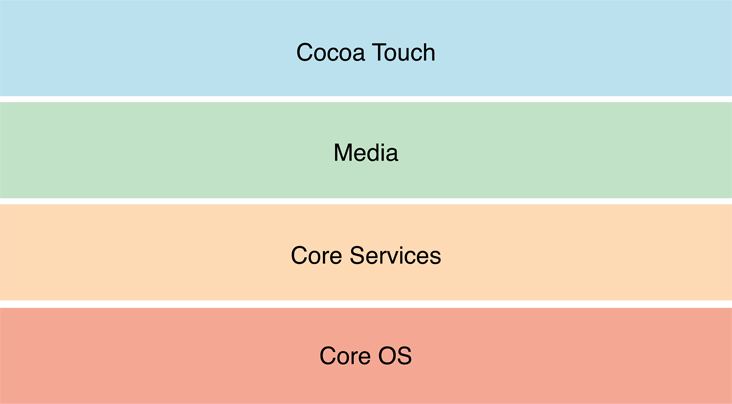
\includegraphics[width=130mm]{fig/ios_layers}
  \caption{Слоистая архитектура \\ операционной системы iOS}
  \label{fig:ios_layers}
\end{figure}

Нижние слои содержат фундаментальные сервисы и технологии.
Слои более высокого уровня опираются на нижние, взаимодействуя с ними,
и обеспечивают доступ к более низкоуровневым сервисам и технологиям.

Слой \textit{Cocoa Touch} содержит ключевые библиотеки для создания iOS-приложений.
Эти фреймворки определяют внешний вид приложений и определяют базовую
инфраструктуру приложений, поддержку ключевых технологий,
таких как многозадачность, сенсорный ввод,
push-уведомления и других высокоуровневых системных сервисов.

Слой \textit{Media} включает в себя графические, аудио- и видеотехнологии,
которые используются для реализации мультимедийных возможностей приложении.

Слой \textit{Core Services} содержит основные системные сервисы. Ключевыми среди
них являются фреймворки Core Foundation и Foundation,
определяющие основные типы, которые используются в приложениях.
Этот слой также включает в себя специфические технологии
для поддержки таких функций, как геолокация, iCloud, сетевые
технологии и другие.

Слой \textit{Core OS} состоит из низкоуровневых функций, на которых базируется
большинство других технологий. Даже если разработчики не используют
эти функции напрямую, они зачастую используются другими библиотеками.
В ситуациях, когда необходимо иметь дело с безопасностью или связью
с аппаратным обеспечением устройства, можно воспользоваться фреймворками этого
слоя.

В процессе создания приложения компания Apple рекомендует отдавать предпочтение
использованию фреймворков более высокого уровня. Библиотеки более высокого
уровня предоставляют собой объектно-ориентированные абстракции
для конструкций более низкого уровня.
Использование библиотек низкого уровня допускается,
если они содержат компоненты, недоступные в фреймворках
более высокого уровня~\cite{ios_core_layers}.

В результате iOS выступает в качестве посредника между низкоуровневым
аппаратным обеспечением устройства и приложениями, которые создают разработчики.
Приложения не взаимодействуют напрямую с аппаратным обеспечением,
они общаются с оборудованием через набор четко определенных системных интерфейсов.
Эти интерфейсы позволяют легко создавать приложения,
которые при этом остаются безопасными для конечного пользователя.

% Xcode & AppCode

Интегрированная среда разработки Xcode --- это пакет средств разработки,
которая используется для создания,
тестирования, отладки и конфигурации iOS-приложений. Среда разработки Xcode
включает в себя приложение Xcode, которое является оболочкой для инструментов
создания приложений, инструменты для отладки и iOS-симулятор.
Для написания и отладки кода используется приложение Xcode,
тестирование происходит путем запуска приложения на iOS симуляторе
или на непосредственно подключенным устройстве под управлением операционной системы iOS.
Для измерения производительности используются инструменты,
которые могут быть запущены из приложения Xcode.

Пользовательский интерфейс среды разработки Xcode представлен
на рисунке~\ref{fig:xcode}.
\begin{figure}[h!]
  \centering
  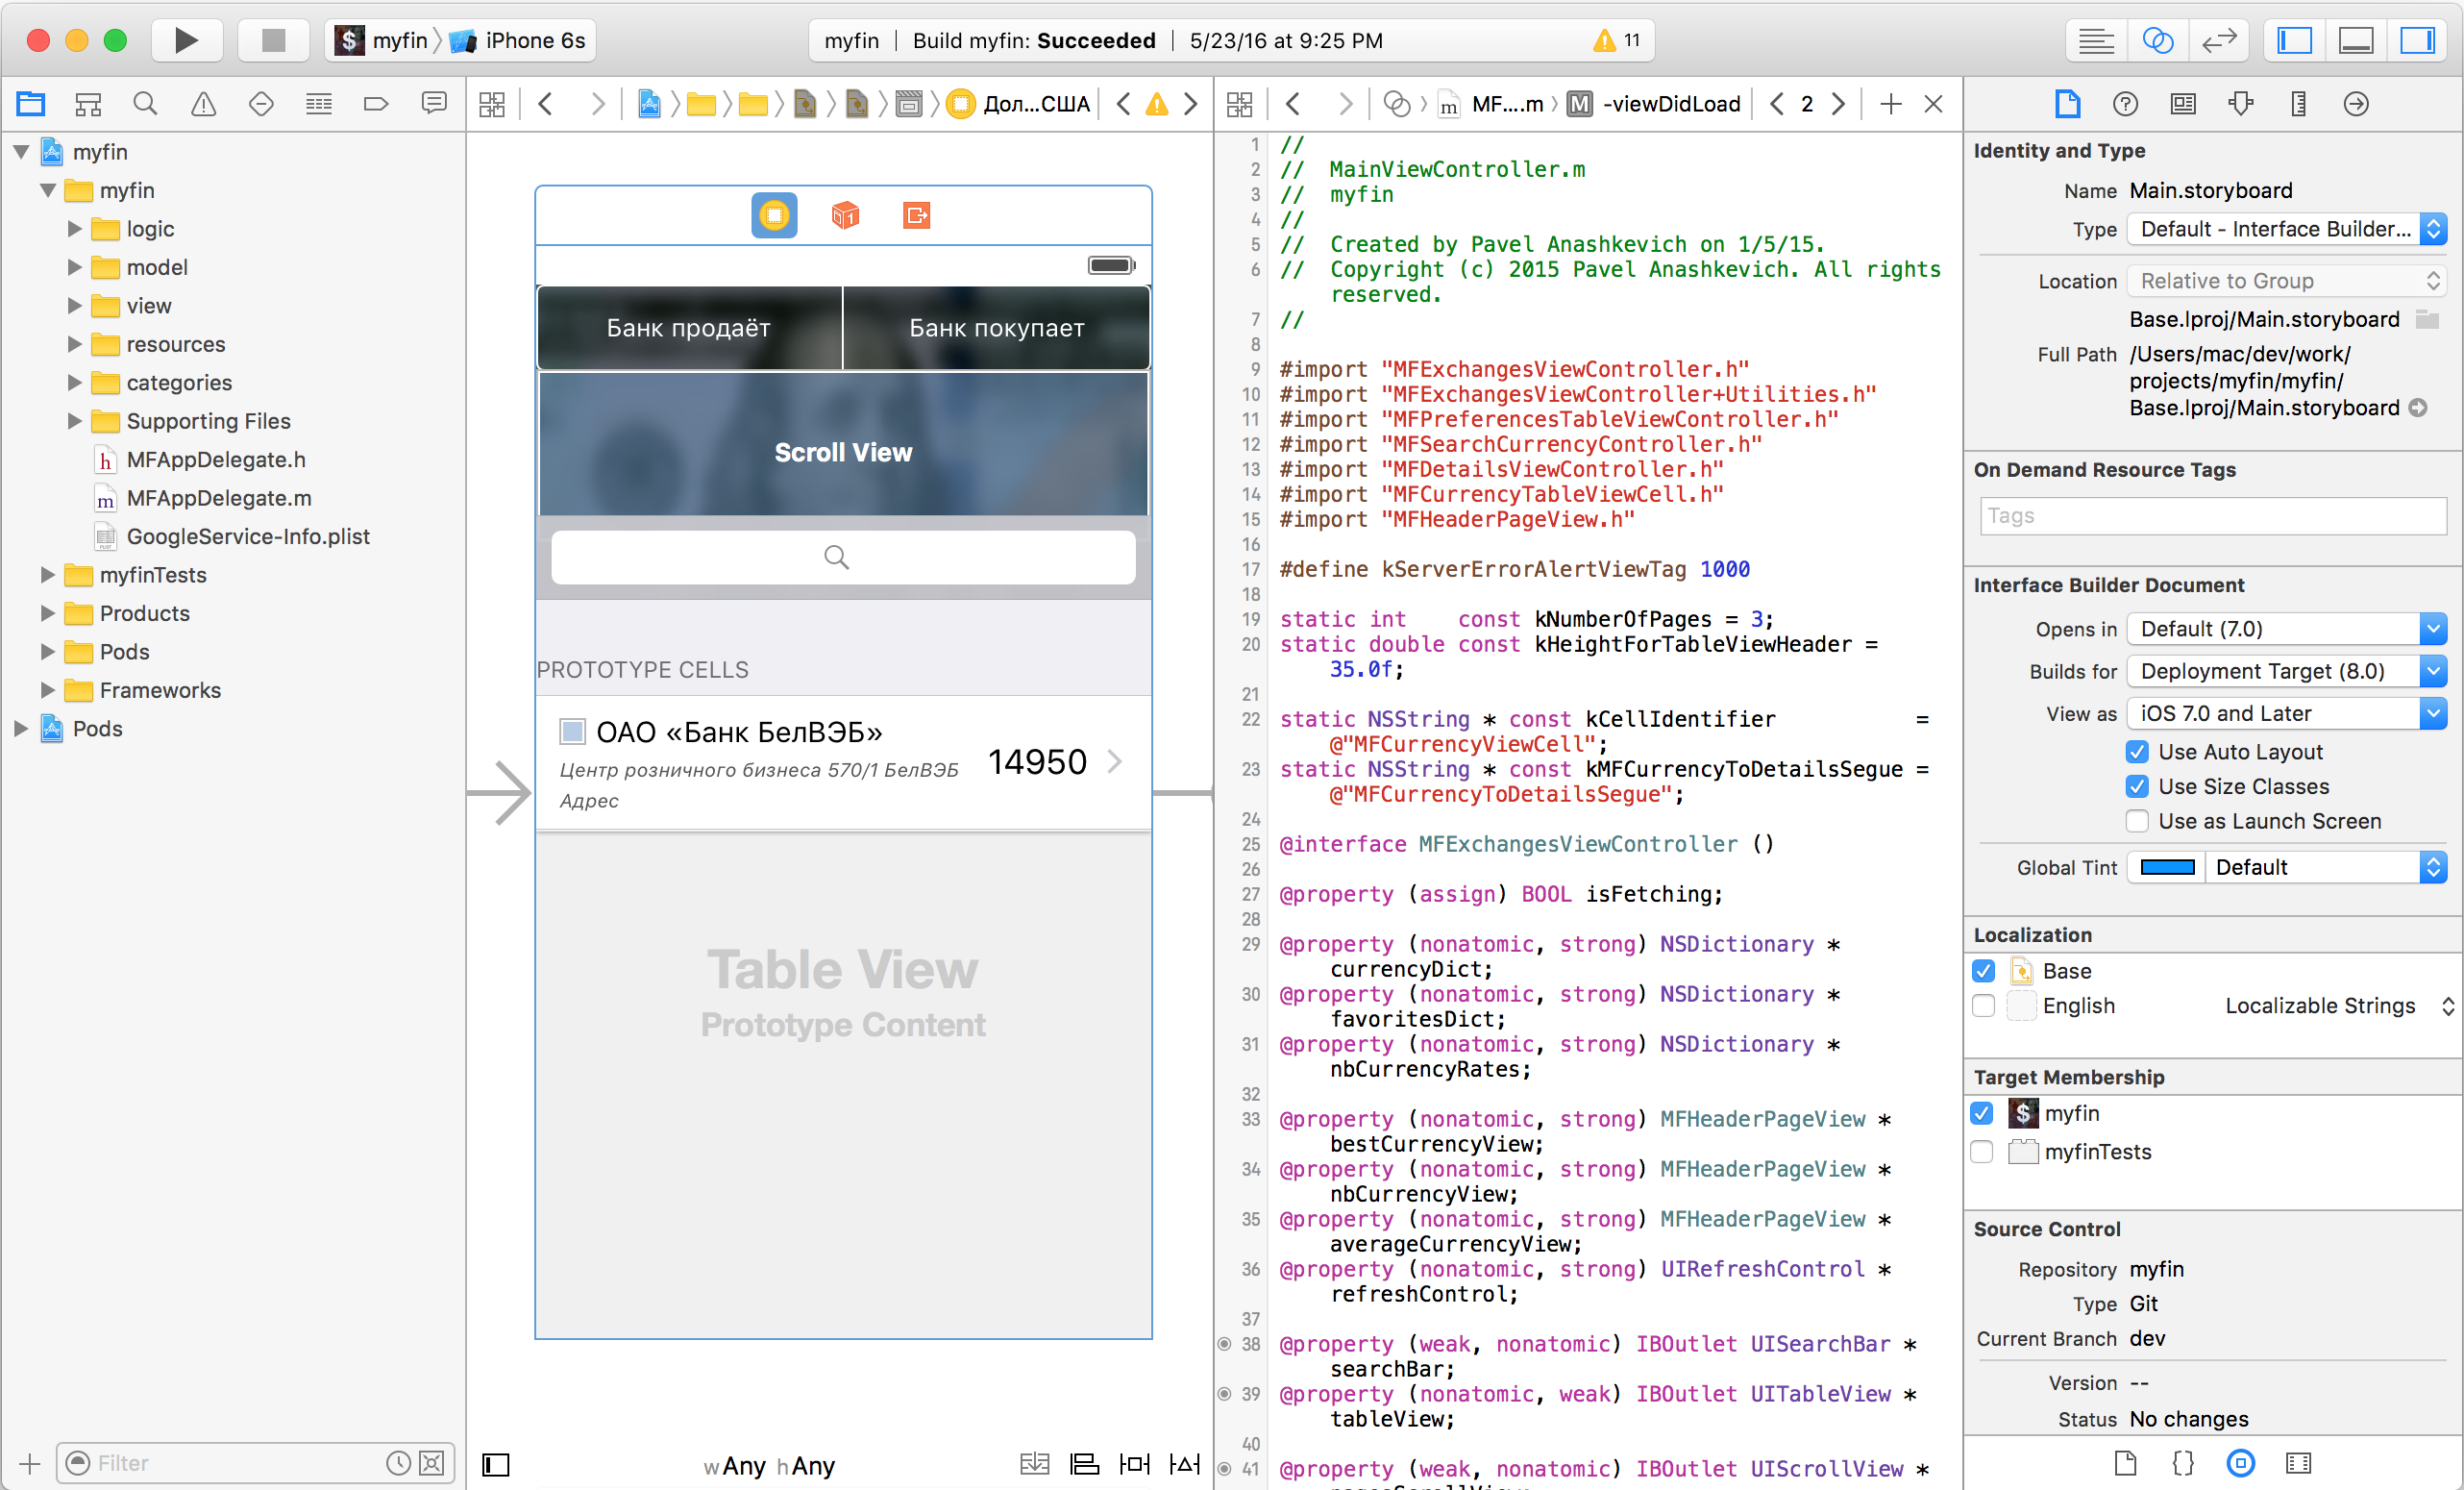
\includegraphics[width=150mm]{fig/xcode}
  \caption{Пользовательский интерфейс \\ среды разработки Xcode}
  \label{fig:xcode}
\end{figure}

Среда разработки Xcode включает в себя ряд возможностей, среди которых:
\begin{itemize}
  \item встроенный редактор Interface Builder для создания пользовательского
    интерфейса приложения;
  \item расширенная подсветка синтаксиса;
  \item использование официальной документации Apple непосредственно в среде разработки;
  \item система сборки проекта, проверка зависимостей;
  \item компиляция кода с использованием LLVM и Clang;
  \item статический анализатор для контроля поведения приложения и выявления
    потенциальных проблем;
  \item комплексная отладка приложения с использованием дебаггера lldb.
\end{itemize}

Стоит отметить, приложение Xcode не является монополистом на рынке
интегрированных сред разработки программных продуктов для платформы iOS и OS X.
Весной 2013 года компания JetBrains представила IDE для создания приложений для
устройств Apple. По словам разработчиков, AppCode призвана облегчить
повседневную работу программистам, разрабатывающим на Objective-C и Swift
приложения для устройств Apple, таких как Mac, iPhone, iPad, Apple Watch и Apple TV.
Для повышения их продуктивности среда разработки AppCode тесно интегрируется с приложением
Xcode и сосредоточена на обеспечении качества кода за счет удобной
навигации по коду, оптимизированному автодополнению, анализу кода
на лету (с мгновенным исправлением обнаруженных проблем)
и автоматизированному рефакторингу.

Пользовательский интерфейс среды разработки AppCode представлен
на рисунке~\ref{fig:appcode}.
\begin{figure}[h!]
  \centering
  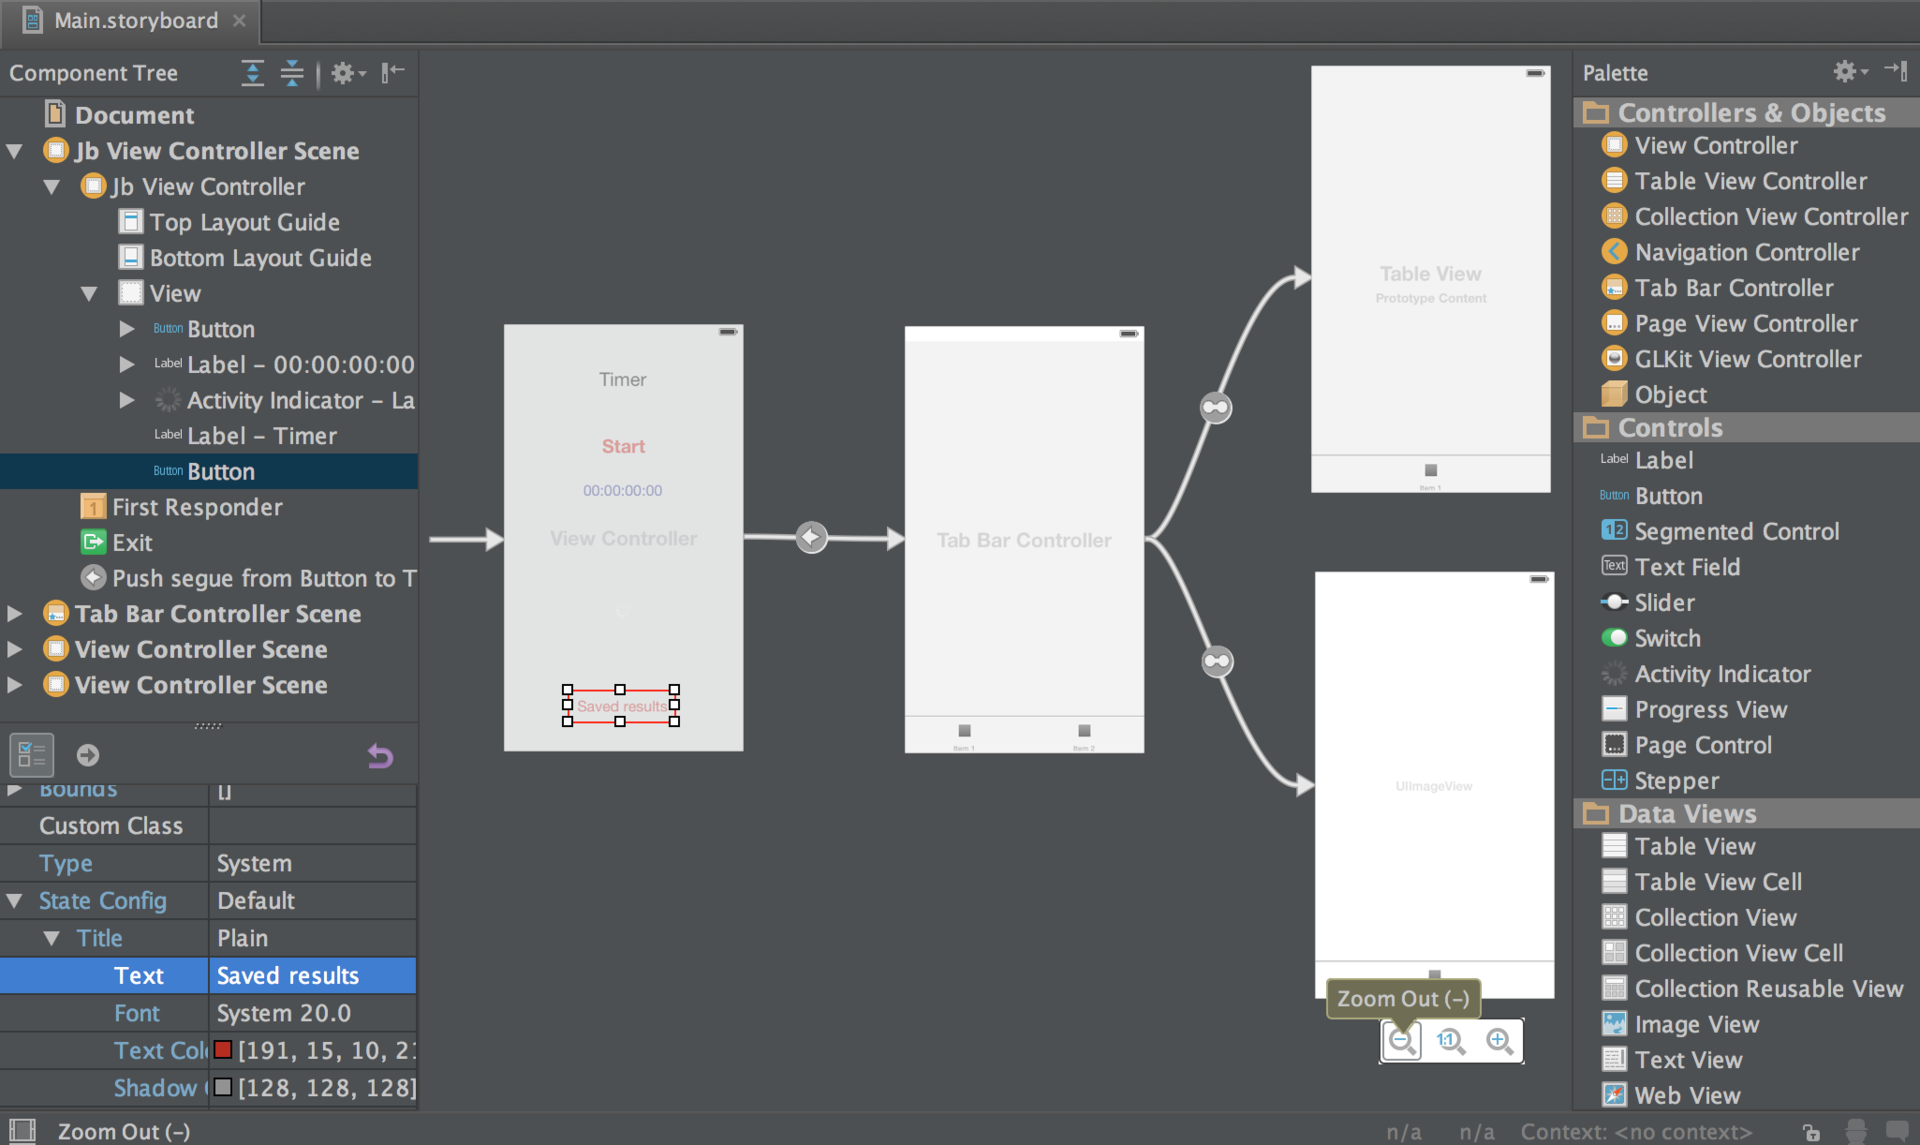
\includegraphics[width=150mm]{fig/appcode}
  \caption{Пользовательский интерфейс \\ среды разработки AppCode}
  \label{fig:appcode}
\end{figure}

Несмотря на большое количество достоинств интегрированной среды разработки AppCode,
не стоит воспринимать её как альтернативу приложению Xcode, так как
IDE от JetBrains не гарантирует полноценную поддержку приложений, написанных с
использованием Xcode. Зачастую разработкам iOS приложений, предпочитающим линейку
продуктов от JetBrains, приходится использовать две среды разработки для одного проекта.
Как правило, в таком случае разработчики используют Xcode для создания
пользовательских интерфейсов с использованием инструмента Interface Builder,
работы с мобильной базой данных CoreData, а написание кода приложения, а также
его отладку производят в интегрированной среде разработки AppCode.

Стоит отметить, что интегрированная среда разработки от JetBrains AppCode
является проприетарным программным обеспечением. Стоимость лицензионной версии AppCode
для индивидуального разработчика составляет приблизительно девяноста
долларов США в год, тогда как IDE Xcode от Apple распространяется через магазин
приложений AppStore на бесплатной основе.

Основными языками программирования, на которых ведётся разработка приложений для
устройств Apple являются Objective-C и Swift.

% Objective-C

Objective-C был придуман Брэдом Коксом в начале 1980-x годов
в качестве модификации языка программирования С в сторону Smalltalk.
Целью Кокса было создание языка, поддерживающего концепцию software IC.
Под этой концепцией понимается возможность собирать программы из готовых
компонент (объектов), подобно тому как сложные электронные устройства могут быть
легко собраны из набора готовых интегральных микросхем (IC, integrated circuits).
Эта модификация состояла в добавлении новых синтаксических
конструкций и специальном препроцессоре для них (который, проходя по коду
преобразовывал их в обычные вызовы функций С),
а также библиотеке времени выполнения (эти вызовы обрабатывающей).
Таким образом, изначально Objective-C воспринимался как надстройка над C.
В каком-то смысле это так и до сих пор: можно написать программу на чистом С,
а после добавить к ней немного конструкций из Objective-C (при необходимости),
или же наоборот, свободно пользоваться С в программах на Objective-C.

В 1988 году компания NeXT (а в последствии Apple)
лицензировала Objective-C и написала для него компилятор и
стандартную библиотеку (SDK).
В 1992 году к усовершенствованию языка и компилятора подключились разработчики
проекта GNU в рамках проекта OpenStep. С тех пор компилятор GCC поддерживает Objective-C.
После покупки NeXT, Apple взяла их SDK (компилятор, библиотеки, IDE) за основу
для своих дальнейших разработок. IDE для кода назвали Xcode,
а для GUI --- Interface Builder.
Фреймворк Cocoa, используемый в основном для разработки графического интерфейса пользователя,
на сегодняшний день является наиболее значимой средой разработки программ на Objective-C.

Файлы модулей на языке Objective-C имеют расширение \textit{.m}
(если использовалась смесь С++ и Objective-С, то расширение \textit{.mm}),
заголовочные файлы --- \textit{.h}. Все создаваемые в Objective-С объекты классов
должны размещаться в динамической памяти. Поэтому особое значение приобретает
тип \textit{id}, который является указателем на объект любого класса (\textit{void *}).
Нулевой указатель именуется константой \textit{nil}.
Таким образом, указатель на любой класс можно привести к типу \textit{id}.
Возникает проблема: как узнать к какому классу относится объект,
скрывающийся под \textit{id}? Это делается благодаря инварианту \textit{isa},
который присутствует в любом объекте класса, унаследовавшего специальный
базовый клас \textit{NSObject} (приставка NS обозначает NeXT Step).
Инвариант \textit{isa} относится к зарезервированному типу \textit{Class}.
Объект такого типа позволяет узнавать имена своего и базового класса,
набор инвариантов класса, а также прототипы всех методов,
которые реализовал этот объект и их адреса (посредством локального списка селекторов).
Все зарезервированные слова Objective-C, отличающиеся от зарезервированных
слов языка С, начинаются с символа \@ (например \textit{@protocol, @selector, @interface}).
Обычно имена инвариантов классов с ограниченной
областью видимости (\textit{@private, @protected}) начинаются с
символа подчеркивания~\cite{objective_c_from_scratch, appledoc_ios}.


% Swift

В 2014 году на конференции The Apple Worldwide Developers Conference Apple
представила язык программирования Swift --- новый язык программирования
для разработки iOS и OS X приложений, который сочетает в себе все лучшее от C и Objective-C,
но лишен ограничений, накладываемых в угоду совместимости с C.
В Swift используются паттерны безопасного программирования и добавлены
современные функции, превращающие создание приложения в простой,
более гибкий и увлекательный процесс. Swift, созданный с чистого листа, ---
это возможность заново представить себе, как разрабатываются приложения.

На разработку нового языка программирования у Apple ушло около четырёх лет.
Основой нового языка программирования послужили существующие компилятор,
отладчик и фреймворки. Разработчики языка упростили процесс управления памятью
с помощью механизма автоматического подсчета ссылок --- Automatic Reference Counting (ARC).
Фреймворки также подверглись серьезной модернизации. Objective-C начал
поддерживать блоки, литералы и модули --- все это создало благоприятные условия
для внедрения современных технологий. Именно эта подготовительная работа
послужила фундаментом для нового языка программирования,
который будет применяться для разработки будущих программных продуктов для Apple.

Swift вобрал в себя всё лучшее от современных языков и разработан с учетом
обширного опыта компании Apple. Компилятор для Swift --- синоним производительности,
язык оптимизирован для разработки без оглядки на компромиссы.
Он спроектирован таким образом, чтобы вы смогли легко разработать
и ваше первое приложение \textit{«hello, world!»}, и даже целую операционную систему.
Все это делает Swift важным инструментом для разработчиков и для самой компании Apple.
Эффективность и простота Swift дают программистам стимулы к обучению,
к тому же теперь они могут распространять свои идеи повсюду:
от мобильных устройств до облачных систем~\cite{about_swift, swift_becomes_open_source}.

Swift работает в 2,6 раза быстрее, чем Objective-C. Apple включила поддержку
динамических библиотек, которые потребляют меньше ресурсов системы и поставляются,
обновляются отдельно от исполняемых файлов приложений.
В результате готовая программа занимает меньше памяти на устройстве.

В декабре 2015 года, вместе с выходом второй версией языка, компания Apple
объявила от открытии исходного кода Swift.
По словам Федериги, вице-президент Apple по разработке ПО, язык Swift уже
стал самым популярным среди разработчиков на веб-хостинге GitHub.
И создатели Swift сейчас активней всех остальных общаются со сторонними разработчиками.
Внутри самой компании программисты стараются максимально использовать Swift
в своей работе. Это и команда разработчиков iCloud, и разработчики OS X,
которые переводят некоторые аспекты платформы на новый язык (к примеру,
управление окнами). По мнению многих, этот простой язык более практичен в разработке.
Благодаря открытому исходному коду Swift теперь можно внедрять
в школы в качестве базы для обучения программированию. Об этом же говорил
и Тим Кук, посетив лекцию <<Hour of Code>> в нью-йоркском Apple Store.
Федериги даже уверен, что в ближайшие 20 лет Swift станет самым
используемым языком программирования~\cite{federighi_about_swift, habr_swift}.

Язык Swift является совместимым с предыдущим языком Apple Objective-C,
что позволяет разработчикам использовать библиотеки, написанные на Objective-C,
а также вести разработку текущих проектов на новом языке, не ограничиваясь
использованием языка Swift только в новых проектах.

Для обеспечения работы мобильных приложений в оффлайн-режиме требуется
использовать некоторое хранилище данных.

В зависимости от объёма информации, хранение данных может осуществляться
различными способами. Например, если объём информации небольшой, то для
сохранения данных может быть достаточно представить эту информацию
в виде последовательности битов и записать её в файл на жестком диске устройства.
Если же объём информации большой, или же представляет собой набор однотипных данных,
которые легко представить в виде объектов, то имеет смысл сохранять данные
с использованием мобильных баз данных.

Учитывая набор входных данных приложения, рассмотренный в подразделе~\ref{subs:dataware},
целесообразным является использование мобильной базы данных. На сегодняшний день
наиболее распространенными вариантами реализации мобильной базы данных являются:
\begin{itemize}
  \item CoreData;
  \item SQLite;
  \item Realm.
\end{itemize}

CoreData представляет собой высокоуровневую реализацию локальных баз данных от Apple,
которая по средством использования Objective-C или Swift функций
выполняет запросы к базе данных SQLite.

Несмотря на наличие высокоуровневого интерфейса для использования SQLite,
возникают случаи, когда необходимо работать с базой данных SQLite напрямую.
Потребность в таком подходе может возникнуть при оперировании очень большими
объёмами данных, где крайне важна оптимизация в выполняемых SQL-запросах.

В 2015 году была представлена кроссплатформенная мобильная база данных Realm.
Realm была создана, чтобы стать лучше и быстрее, чем SQLite и Core Data.
Действительно, например, запросы подсчёта записей в таблице по запросу,
выполняются примерно в 2 раза быстрее, чем с использованием SQLite,
а по сравнению с CoreData разница в скорости выполнения операций составляет
приблизительно 15 раз~\cite{core_data_diff, core_data_vs_sqlite}.

Мобильная база данных Realm является не только высокопроизводительной,
но и достаточно простотой в использовании, так, разработчикам предоставляется возможность
сделать многое с помощью всего нескольких строк кода. Realm является
совершенно бесплатной, можно использовать ее без каких-либо ограничений~\cite{todo_swift_realm}.


Таким образом, благодаря покрытию абсолютно всех этапов разработки приложения,
в качестве среды разработки программного модуля будет использована IDE Xcode,
языки программирования --- Objective-C и Swift.
В качестве хранилище данных будет использована кросс-платформенная мобильная
база данных Realm, так она сочетает в себе высокую производительность,
удобство использования, а также высокую надёжность выполняемых операций.

\pagebreak


% Реализация структуры программного модуля

\subsection{Реализация структуры программного модуля}

С учётом постановки задачи, изложенной в подразделе~\ref{subs:task_definition},
а также основанной но ней диаграмме декомпозиции верхнего уровня,
проиллюстрированной на рисунке~\ref{fig:idef0}, разрабатываемое
приложение следует разделить на подсистемы, у каждой из которых будут
определенные функциональные обязанности.

Так, например, при наиболее очевидном варианте использования приложения,
можно выделить следующие функциональные блоки системы:
\begin{itemize}
  \item загрузка данных с внешних серверов или из БД (ввод данных);
  \item выбор валюты (по умолчанию осуществляется автоматически);
  \item подготовка данных для отображения (фильтрация, сортировка);
  \item вывод данных на экран.
\end{itemize}

Для наглядного отображения приведём структура программного модуля,
разделенного на подсистемы в виде диаграммы, построенной по методологии IDEF0.
Диаграмма декомпозиция программного модуля приведена
на рисунке~\ref{fig:idef0_structure}.
\begin{figure}[h!]
  \centering
  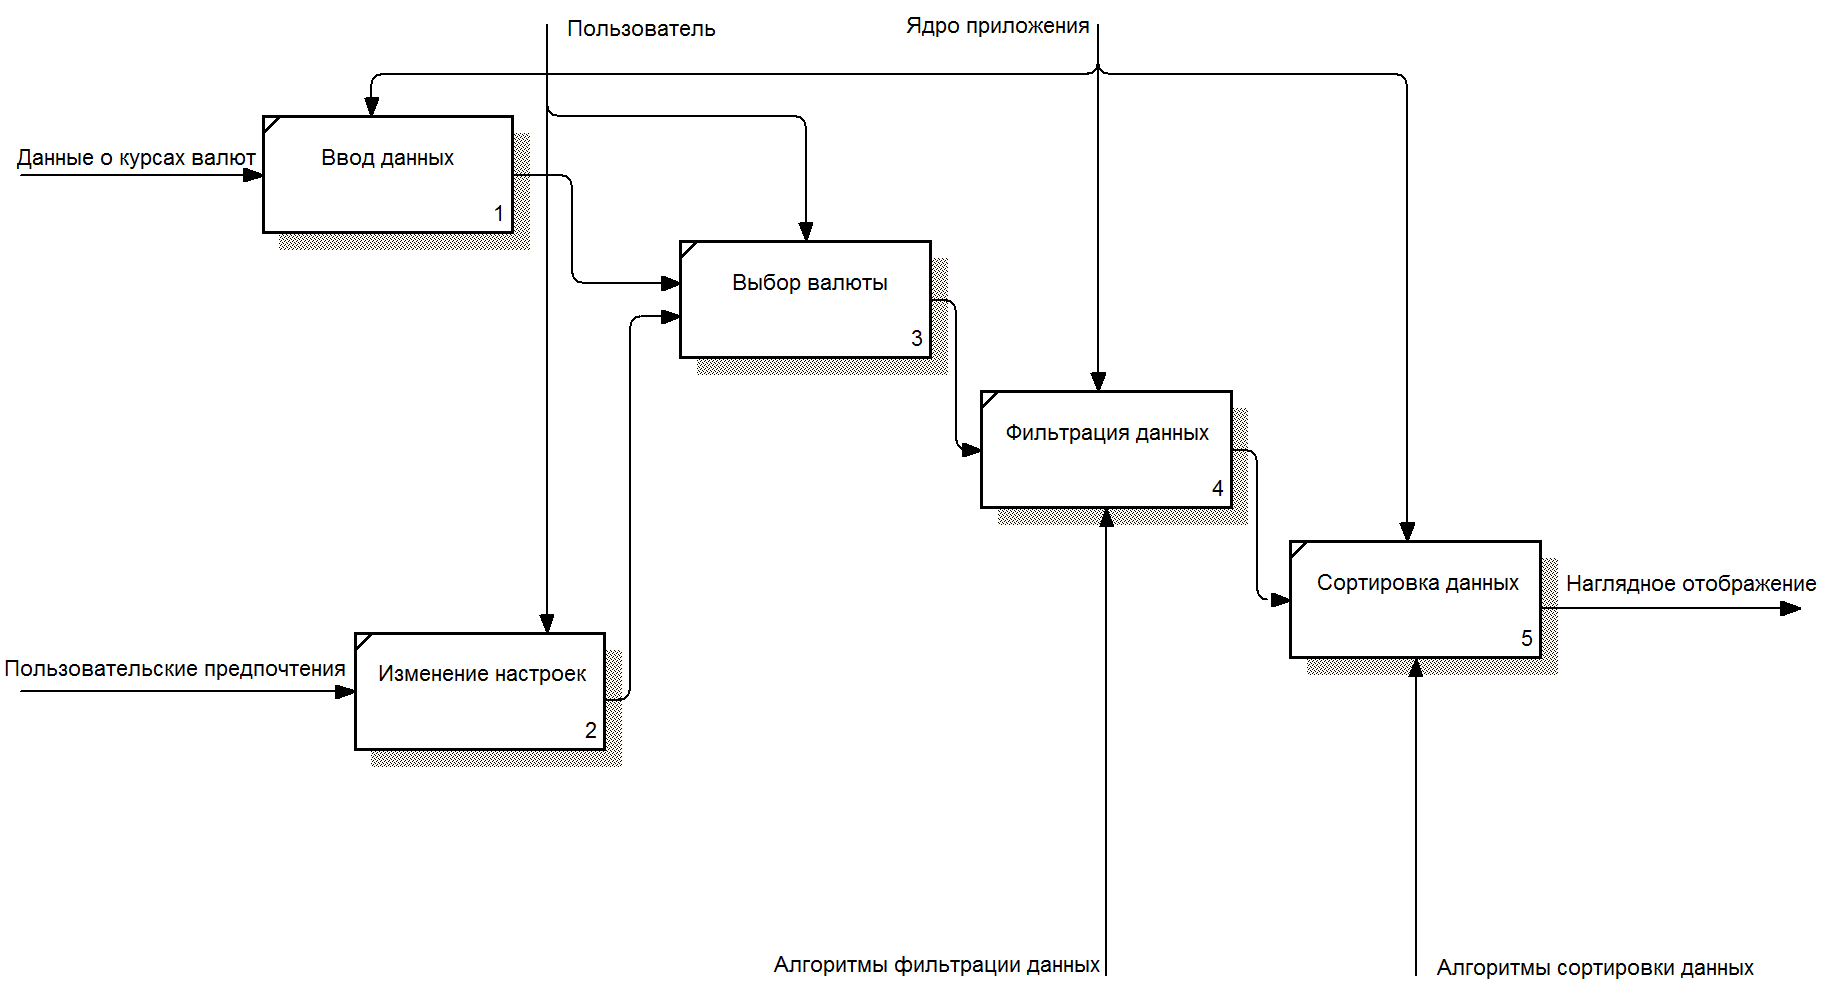
\includegraphics[width=165mm]{fig/IDEF0_structure}
  \caption{Диаграмма декомпозиции программного модуля}
  \label{fig:idef0_structure}
\end{figure}

\newpage


% Реализация подсистемы загрузки данных

\subsection{Реализация подсистемы загрузки данных}
\label{subs:realization_network_requests}

Подсистема загрузки данных приложения представляет собой независимый блок,
на вход которому поступает адрес интерфейса прикладного программирования (API),
выходом служат данные, готовые для дальнейшей обработки и сохранения
в мобильной базе данных.

Адрес API финансового портала myfin.by является параметрическим,
в качестве параметра выступает уникальный код областного центра Республики Беларусь.
Таким образом, построение результирующего URL выполняется путём конкатенации
статической строки адреса API и кода областного центра.
Соответствие областных центров конечным URL сведены в таблицу~\ref{tbl:url_by_city}.
\begin{table} [h!]
  \caption{
    Соответствие наименований областных центров конечным \\
    \hspace{29.5mm} URL финансового портала myfin.by
  }\label{tbl:url_by_city}
    \begin{tabular}{| m{4.75cm} | c | c |}
      \hline

      Наименование \newline областного центра & Код  города & Конечный URL \\
      \hline

      г. Минск    & 1 & http://admin.myfin.by/outer/authXml/1 \\ \hline
      г. Витебск  & 2 & http://admin.myfin.by/outer/authXml/2 \\ \hline
      г. Гомель   & 3 & http://admin.myfin.by/outer/authXml/3 \\ \hline
      г. Гродно   & 4 & http://admin.myfin.by/outer/authXml/4 \\ \hline
      г. Брест    & 5 & http://admin.myfin.by/outer/authXml/5 \\ \hline
      г. Могилёв  & 6 & http://admin.myfin.by/outer/authXml/6 \\ \hline

    \end{tabular}
\end{table}

Стоит отметить, что доступ к приведенным в таблице~\ref{tbl:url_by_city} адресам
ограничен. Существует два варианта получение доступа со стороны финансового портала:
использование выделенного (статического) IP-адреса, или же http-запрос,
включающий в себя процесс авторизации. Учитывая то, что разрабатываемый
программный модуль в широком смысле является приложением-клиентом,
которое будет запускаться на различных устройствах,
то использование статического IP-адреса становиться невозможным. В результате,
по договорённости с финансовым порталом myfin.by, для разрабатываемого
программного модуля был выделен логин и пароль, с помощью которого будет
выполнятся http-запрос с авторизацией.

Для получения данных о курсах валют, установленных Национальным банком Республики
Беларусь, требуется выполнить параметрический запрос:

\textit{http://www.nbrb.by/Services/XmlExRates.aspx?ondate=\{date\}}, \\
где в качестве параметра \textit{date} выступает дата, записанная в определённом
формате.

Обращая внимание на количество аналогичных http-запросов, а также их схожесть
(запросы являются параметрическими, ответом на запрос выступают данные в формате XML,
или информация об ошибке), целесообразным является создание интерфейса выполняемых
сетевых операций. Для этого в языке Swift используются протоколы.

\textit{Протокол} определяет образец методов, свойств или другие требования,
которые соответствуют определенному конкретному заданию или какой-то функциональности.
Протокол фактически не предоставляет реализацию для любого из этих требований,
он только описывает как реализация должна выглядеть. Протокол может быть принят классом,
структурой или перечислением для обеспечения фактической реализации этих требований.
Любой тип, который удовлетворяет требованиям протокола,
имеет указание соответствовать этому протоколу.

В дополнение к определенным требованиям, которые должны быть реализованы
подписанными под протокол типами, можно также расширить протокол, чтобы реализовать
некоторые из этих требований или для того, чтобы реализовать дополнительную
функциональность, которую смогут использовать подписанные под протокол
типы~\cite{swiftbook_protocols}.

Для определения общего интерфейса выполняемых сетевых операций создадим
протокол \textit{Operation}, который в дальнейшем, будет реализован дочерними классами.
Определение протокола Operation приведено на рисунке~\ref{lst:protocol_operation}.
\lstinputlisting[
    caption=Определение протокола \textit{Operation},
    label=lst:protocol_operation,
]{lst/protocol_operation.lst}

Функция \textit{startWithCompletion:} является основной для протокола Operation,
так как именно её будут реализовывать классы, подписавшиеся на следование
данному протоколу.

Нетрудно заметить, что реализация функции \textit{networkRequestForURL:} для всех
наследников протокола \textit{Operation} будет одинаковой. Таким образом, имеет смысл
реализовать эту функцию на уровне протокола. Это обеспечит
доступ к реализованной функции всем подписчикам протокола \textit{Operation},
без необходимости написания однотипной реализации данной функции.
Реализация функции на уровне протокла (по умолчанию) в языке Swift выполняется с помощью
конструкции расширения.

\textit{Расширения} добавляют новую функциональность существующему типу класса,
структуры или перечисления. Это включает в себя возможность расширять типы,
к исходным кодам которых у вас нет доступа (известно как ретроактивное
моделирование)~\cite{swiftbook_extensions}.

Расширение протокола \textit{Operation} приведено на рисунке~\ref{lst:operation_extension}.
\lstinputlisting[
    caption=Расширение протокола \textit{Operation},
    label=lst:operation_extension,
]{lst/operation_extension.lst}

Приведенная функция \textit{networkRequestForURL:} служит для выполнения сетевых
операций при заданном URL. Блок \textit{completion} служит для обратной связи
с вызывающей функцией и будет вызван тогда, когда сетевая операция завершится.

Таким образом, протокол \textit{Operation}, а также его расширение, позволят
существенно упростить логику, а также выполнение всех сетевые операции
в едином логическом стиле независимо от классов, подписанных на данный протокол.
Классами, которые подписаны на протокол \textit{Operation} являются:
\textit{MyFinOperation}, \textit{NationalBankOperation} и \textit{GeocodeOperation}.

Класс \textit{MyFinOperation} реализует логику сетевого запроса к API
финансового портала myfin.by.

Класс \textit{NationalBankOperation} реализует логику сетевого запроса к API
сайта Национального банка Республики Беларусь.

Класс \textit{GeocodeOperation} используется для преобразования адреса,
представленного в виде строки в координаты широты и долготы.

Реализация функций \textit{startWithCompletion:} и \textit{operationForCity:},
описанных в классе \textit{MyFinOperation}, представлена
на рисунке~\ref{lst:start_with_completion_realization}.
\lstinputlisting[
    caption=Реализация функции \textit{startWithCompletion:},
    label=lst:start_with_completion_realization,
]{lst/start_with_completion_realization.lst}

В приведенной на рисунке~\ref{lst:start_with_completion_realization} функции
выполняется создание отдельного потока для выполнения запроса, а также
последующей обработки информации. Функция \textit{parseMyFinResponse:} выполняет
преобразование полученных с сервера данных в объекты модели данных.

Полный исходный код реализации класса \textit{MyfinOperation} приведен в приложении~А.

\pagebreak


% Реализация подсистемы хранения данных

\subsection{Реализация подсистемы хранения данных}
\label{subs:impl_storage}

Мобильная база данных Realm является объектно-ориентированной,
для сохранение какой-либо информации в ней требуется создание классов
модели данных, унаследованных от класса \textit{Object} модуля \textit{Realm}.
Несмотря на ограниченное количество поддерживаемых типов данных,
Realm обеспечивает полноценное покрытие спроектированной в
подразделе~\ref{subs:dataware} модели данных.

Так, сущности <<Банк>> соответствует класс \textit{Bank}, сущности <<Отделение>>
соответствует класс \textit{Department}, а сущности <<Курс>> ---
класс \textit{ExchangeRates}. Рассмотрим реализацию класса \textit{Bank},
приведенного на рисунке~\ref{lst:bank}, подробнее.
\lstinputlisting[
    caption=Реализация класса модели данных \textit{Bank},
    label=lst:bank,
]{lst/bank.lst}

В приведенном классе описаны поля \textit{id, name, website}, отражающие
уникальный идентификатор банка, название, а также сайт, если
информация о нём предоставлена. Поле \textit{departments} содержит список
отделений конкретного банка. Этот список инициализируется при создании объекта
класса \textit{Bank}, количество элементов в нём может изменяться.

Модификатор \textit{private(set)} служит для ограниченного доступа
к свойствам объекта, таким образом, чтобы они были доступны только для чтения.
Ключевое слово \textit{dynamic} существует для корректной интерпретации и поддержки
времени выполнения языка Objective-C.

Полный исходный код реализации модели данных программного модуля
приведен в приложении~Б.

Очевидно, что отображение получаемых в формате XML данных от API финансового
портала myfin.by в рассматриваемую модель данных в автоматическом режиме
выполнить невозможно. Поэтому, для выполнения данной операции требуется создать
структуру \textit{DepartmentXMLMap}, которая будет являться вспомогательной
на пути преобразования информации из формата XML в объекты модели данных,
пригодные для сохранения в Realm.

Реализация вспомогательной структуры \textit{DepartmentXMLMap} представлена
на рисунке~\ref{lst:departments_xml_map}.
\lstinputlisting[
    caption=Реализация вспомогательной структуры \textit{DepartmentXMLMap},
    label=lst:departments_xml_map,
]{lst/departments_xml_map.lst}

Таким образом, при инициализации приложения будет выполняться загрузка данных с
удаленных API, преобразование этих данных в объекты класса \textit{DepartmentXMLMap}.
При удачном выполнении этих действий, объекты этого класса будут преобразованы в
объекты модели данных и сохранены в мобильную базу данных Realm. Стоит отметить,
что во время выполнения операции загрузки данных с удалённых API могут возникнуть
ошибки. Причинами неудачной загрузки данных с сервера могут стать:
\begin{itemize}
  \item отсутствие интернет-соединения на мобильном устройстве;
  \item потеря интернет-соединения во время загрузки данных;
  \item ошибка на стороне баз данных удаленных серверов и др.
\end{itemize}

В случае возникновения такой ошибки, будет выполнен запрос на получение
необходимой информации из мобильной базы данных ~\textit{Realm}. В том случае, если
полученная из БД информация устарела (с момента последнего обновления прошло
больше суток), пользователь будет оповещен о возможной неактуальности данных,
но будет иметь возможность продолжить работу с программным модулем.

Для удобства работы с мобильной базой данных создадим класс \textit{RealmManager},
который будет представлять собой удобный для работы интерфейс предлагаемых
мобильной базой данных операций по работе с данными. Фрагмент
класса \textit{RealmManager} приведен на рисунке~\ref{lst:realm_manager}.
\lstinputlisting[
    caption=Фрагмент класса \textit{RealmManager},
    label=lst:realm_manager,
]{lst/realm_manager.lst}

В результате сохранение полученных объектов класса \textit{Bank} в мобильную
базу данных может быть выполнено с использованием команды:

\textit{RealmManager.sharedManager.writeObjects(banks)}

Аналогичными командами может выполняется чтение, а также обновление информации
в мобильной базе данных \textit{Realm}.

Для удобства работы с множеством кодов областных центров Республики Беларусь,
имеет смысл создать перечисление. Для этого в языке Swift существует
конструкция \textit{Enum}.
Перечисления определяют общий тип для группы связанных значений и позволяют
работать с этими значениями в типобезопасном режиме.

Исходный код перечисления \textit{City} представлен на рисунке~\ref{lst:city_enum}.
\lstinputlisting[
    caption=Реализация перечисления \textit{City},
    label=lst:city_enum,
]{lst/city_enum.lst}

Благодаря широким возможностям перечислений в языке Swift, а именно
возможности использования функций, вычисляемых полей, получение URL в
зависимости от областного центра заметно упрощается. Так, используя объект
перечисления \textit{City}, для получения правильного URL достаточно
будет вызвать функцию \textit{myfinURL:} этого объекта.


% Реализация подсистемы отображения информации

\subsection{Реализация подсистемы отображения информации}

Разработка нативных приложений для платформы iOS предполагает использования
библиотеки \textit{UIKit}, разработанной компанией Apple. Эта библиотека представляет
собой набор спецификация для создания графического интерфейса пользователя.

Базовой сущностью библиотеки \textit{UIKit} является элемент представления \textit{UIView}.
Сущность \textit{UIViewController} предоставляет интерфейс для управления отображением
элементов представления на экран устройства. Одному экрану приложения соответствует
одна сущность \textit{UIViewController}, в результате выполняется разделение
логики приложения по этим сущностям, а также их вспомогательным файлам --- сервисам.

Для грамотного построения логики приложения, а также корректной реализации графического
интерфейса пользователя, важно понимать жизненный цикл сущности \textit{UIViewController},
который представлен на рисунке~\ref{fig:vc_lifecycle}.
\begin{figure}[h!]
  \centering
  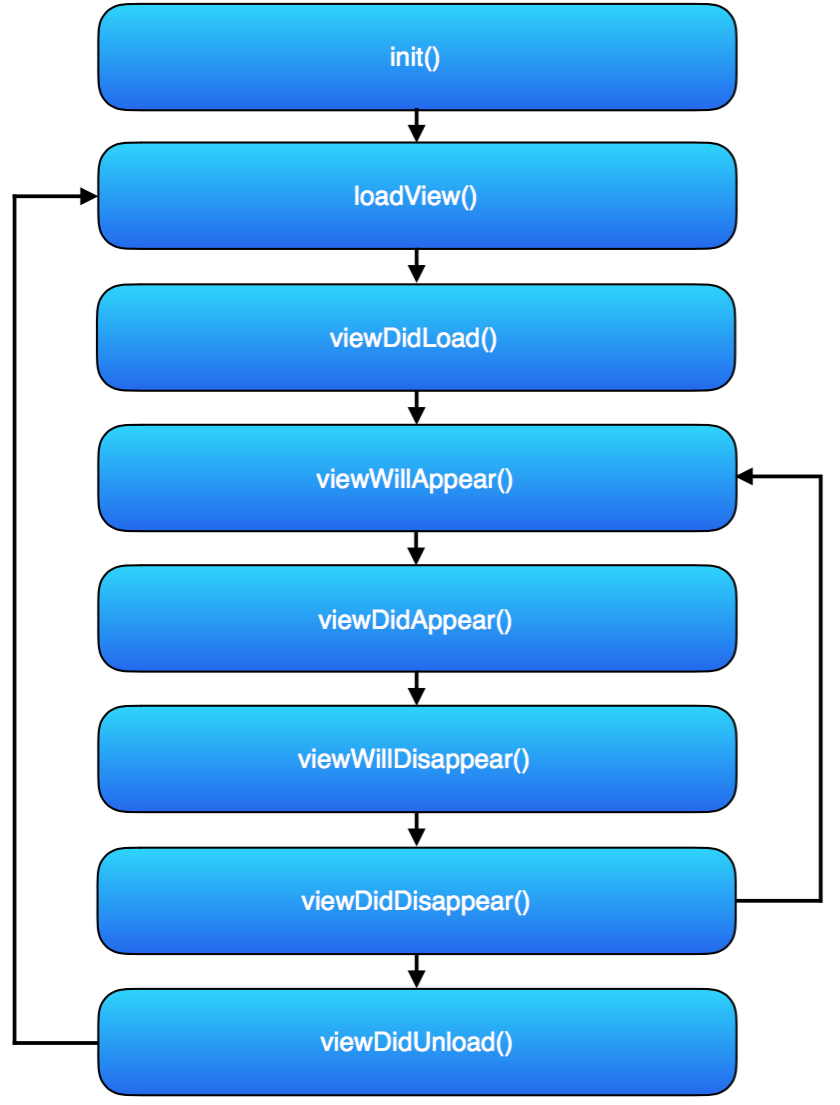
\includegraphics[width=107mm]{fig/vc_lifecycle}
  \caption{Жизненный цикл сущности \textit{UIViewController}}
  \label{fig:vc_lifecycle}
\end{figure}

Сложно выделить наиболее важные функции жизненного цикла сущности \textit{UIViewController},
однако наиболее используемыми из них являются \textit{viewDidLoad()},
\textit{viewWillAppear()}, а также \textit{viewDidDisappear()}.

Функция \textit{viewDidLoad()} вызывается в момент полной загрузки
сущности \textit{UIView} в память устройства. В этой момент обычно производят
окончательные настройки пользовательского интерфейса текущего экрана.
Бывают случаи, когда именно в этой функции следует выполнять загрузку каких-либо
данных, одновременно показывая на экране устройства индикатор загрузки.

Функция \textit{viewWillAppear()} вызывается в тот момент, когда в приложении
планируется переход на текущий экран. Как правило, эта функция за время жизни приложения
вызывается гораздо чаще функции \textit{viewDidLoad()}, поэтому не стоит выполнять
в этой функции трудозатратные операции. Однако, при необходимости частого
обновления информации бывает удобно выполнять логику загрузки данных в этой
функции.

Функция \textit{viewDidDisappear()} вызывается в тот момент, когда пользователь
покинул текущий экран приложения и все анимации перехода между экранами завершили
своё действие. В блоке этой функции удобно приостанавливать загрузку данных и
какую-либо анимацию, связанную непосредственно с экраном, который покинул
пользователь.

Главным классом-наследником \textit{UIViewController} в разрабатываемом программном
модуле будет являться класс \textit{CurrencyViewController}, который будет
ответственен за управление отображением списка отделений выбранной пользователем
валюты, а также дополнительным полем, на котором будут отображаться основные
значения, связанные с текущей валютой (лучшее, среднее значение обмена валют,
курс валют, установленный Национальным банком Республики Беларусь).

Выбор валюты пользователем может быть осуществлен с помощью элемента \textit{UITabBar}
библиотеки \textit{UIKit}, представляющего собой поле, расположенной в нижней
части экрана, на котом расположены пять кнопок, соответствующие определенной валюте.
Визуальный элемент выбора валюты \textit{UITabBar} представлен на
рисунке~\ref{fig:tabbar}.
\begin{figure}[h!]
  \centering
  
\includegraphics[width=140mm]{fig/tabbar}
  \caption{Визуальный элемент выбора валюты \textit{UITabBar}}
  \label{fig:tabbar}
\end{figure}

По нажатию на любую из представленных на рисунке~\ref{fig:tabbar} кнопок будет
выполнена загрузка информации о соответствующей валюте с отображением
на \textit{UIView}, которой управляет объект класса \textit{CurrencyViewController}.
Перед отображением полученная информация проходит процессы фильтрации
и сортировки. Процесс фильтрации представляет собой процесс отбрасывания
данных об отделениях, информация об обменном курсе валют для выбранной валюте не
предоставляется. Процесс сортировки представляет собой сортировку данных
по значению курса обмена валют от наилучшего к наихудшему.

Очевидно, что если пользователь предполагает сдать
валюту (продать банку), то наилучшим значением
является максимальное значение обменного курса, и наоборот, если пользователь
планирует купить валюту, то наилучшим значением будет являться минимальная
величина обменного курса данной валюты.

Пользовательский интерфейс главного экрана приложения представлен на
рисунке~\ref{fig:main_screen}.
\begin{figure}[h!]
  \centering
  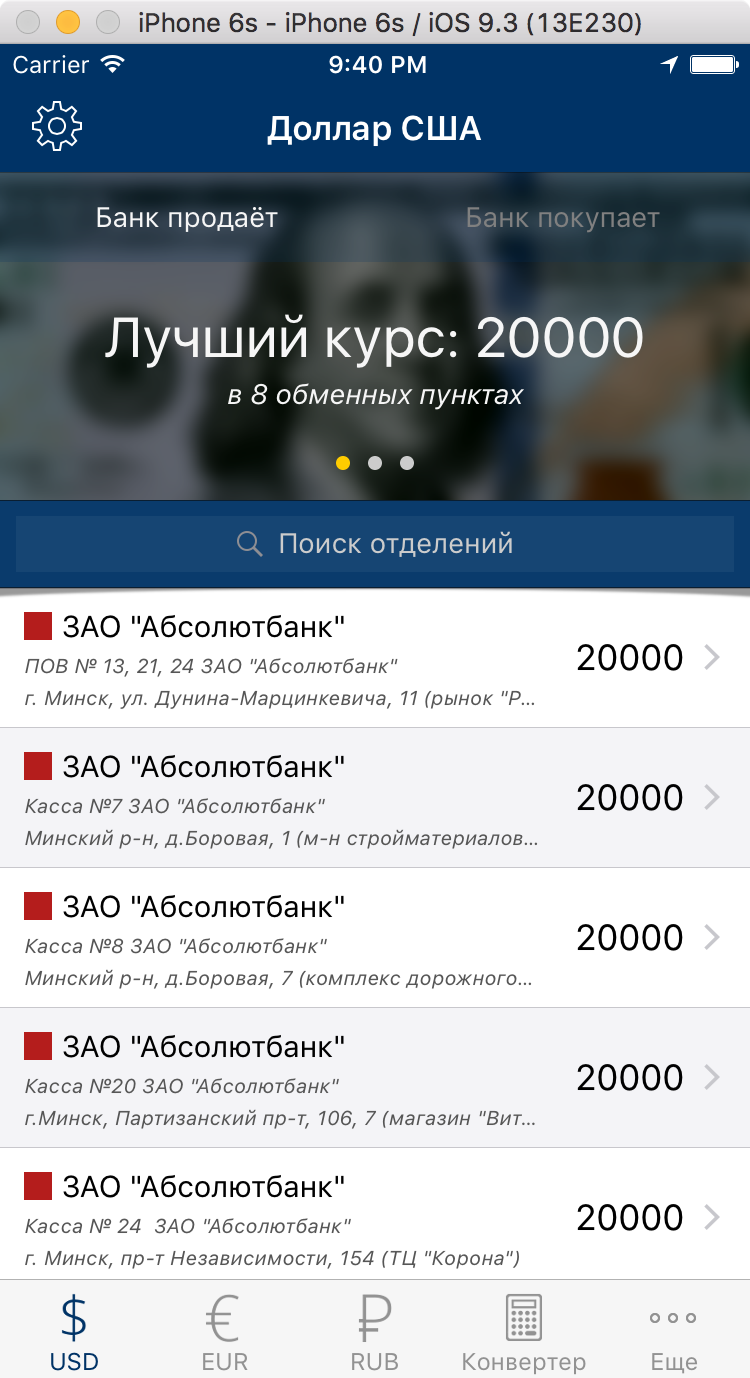
\includegraphics[width=65mm]{fig/main_screen}
  \caption{Снимок главного экрана \\ программного модуля}
  \label{fig:main_screen}
\end{figure}

\pagebreak

Для отображения детальной информации об отделении целесообразно создать отдельный
экран, на который имеется возможность перейти несколькими способами. Первым,
наиболее очевидным для пользователей платформы iOS, будет переход к детальной
информации об отделении по нажатию на поле отделения в списке.

На экране отображения детальной информации об отделении будет представлена
следующая информация:
\begin{itemize}
  \item название банка (заголовок экрана);
  \item название отделения;
  \item адрес отделения;
  \item телефон отделения;
  \item сайт банка;
  \item курсы валют, установленные в отделении.
\end{itemize}

С целью наглядного отображения местоположения отделения имеет смысл показать
его на карте. Для этого в разрабатываемом программном модуле используется
сторонняя библиотека \textit{GoogleMaps}. С помощью \textit{Google Maps SDK}
можно добавлять в приложение карты на основе данных Google Карт.
Пакет SDK автоматически управляет доступом к серверам Google Карт,
отображением карты и реакцией на действия пользователя (например, на нажатия
и перетаскивания объектов). На карту можно добавлять маркеры,
ломаные линии, наземные наложения и информационные окна. Эти объекты
предоставляют дополнительную информацию о местоположениях на карте и
обеспечивают возможности взаимодействия пользователей с
картой~\cite{google_maps_ios}.

Для отображения отделения на карте, необходимо знать его координаты:
широту и долготу. Учитывая то, что источник данных о коммерческих
банках не предоставляет данной информации, требуется использовать сервис геокодирования.

Геокодирование --- процесс преобразования адресов в географические
координаты (широту и долготу), которые можно использовать для размещения
маркеров на карте или ее позиционирования.
Обратное геокодирование~--- это процесс преобразования географических координат
в адреса, понятные для пользователя. Представленная в \textit{Google Maps Geocoding API}
служба обратного геокодирования также позволяет найти адрес по указанному
идентификатору места~\cite{google_geocoding}.

В результате в момент загрузки детальной информации об отделении будем выполнять
запрос к службе геокодирования от \textit{Google}. Результатом запроса будут
координаты отделения банка, которые будут использованы для отображения отделения
на карте.

\newpage

Вспомогательным модулем приложения является конвертер валют. Он предоставляет
пользователю интуитивно-понятный интерфейс для конвертации валют с использованием
курсов, установленных как Национальным банком Республики Беларусь, так и
коммерческими банками.
Пользовательский интерфейс экрана <<Конвертер валют>> представлен на
рисунке~\ref{fig:converter_screen}.
\begin{figure}[h!]
  \centering
  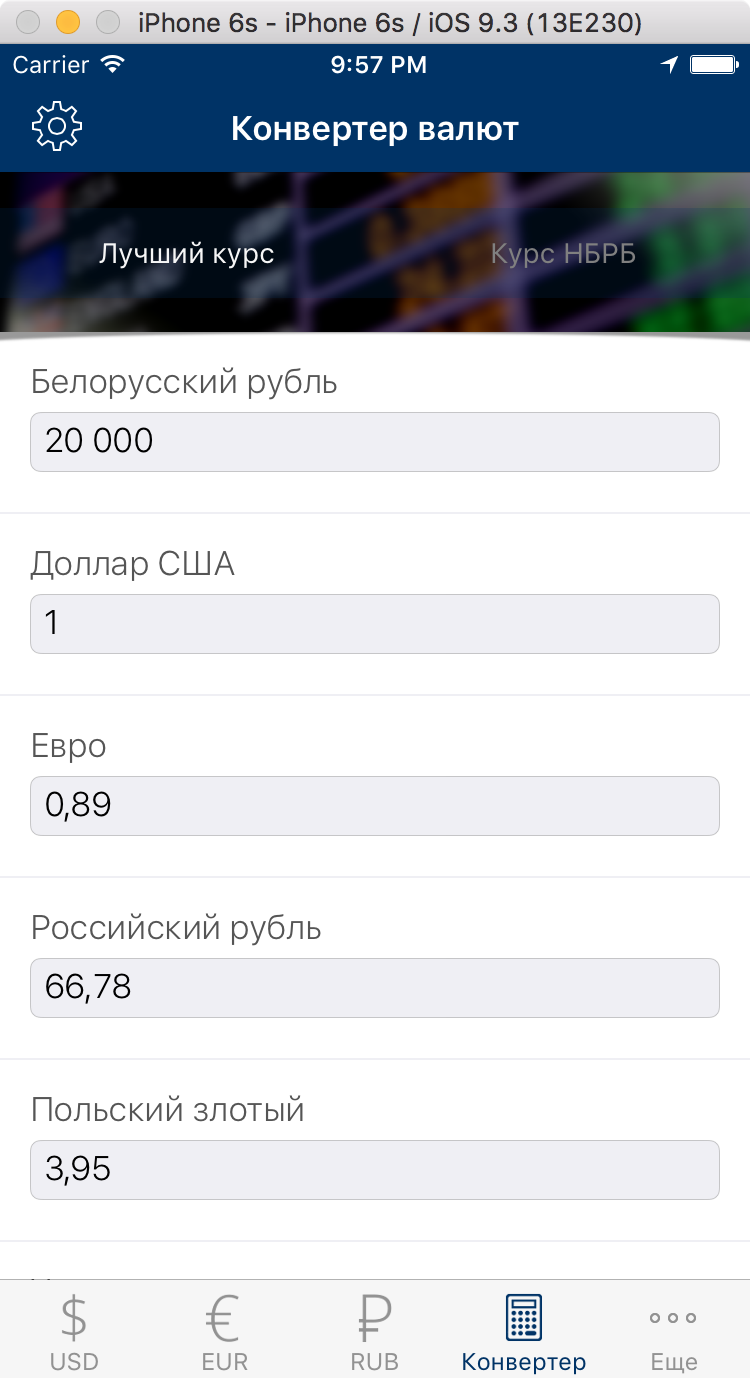
\includegraphics[width=75mm]{fig/converter_screen}
  \caption{Снимок экрана \\ <<Конвертер валют>>}
  \label{fig:converter_screen}
\end{figure}

По нажатию на поле, в котором записано значение курса валют по умолчанию,
открывается виртуальная цифровая клавиатура. Таким образом, пользователь имеет
возможность ввести необходимое значение для конвертации. При изменении текущего
поля все остальные поля со значениями соответствующих курсов валют
автоматически пересчитываются.


% Руководство пользователя

\subsection{Руководство пользователя}

Для использования приложения требуется загрузить его из магазина
приложений \textit{App Store}, перейдя по ссылке~\cite{itunes_app_link},
или же набрав в строке поиска запрос <<курсы валют в Республике Беларусь>>.
Для корректной работы приложения во время первого запуска устройство
под управлением iOS должно быть подключено к сети Интернет.

Рассмотрим возможные варианты использования приложения в соответствии с
представленной на рисунке~\ref{fig:use_case} диаграммой прецедентов.


% Обычный просмотр курсов валют. Выбор валюты.

\paragraph{}
Пользователь имеет возможность просматривать курсы валют в отделениях в списке.
Для этого достаточно запустить приложение: откроется главный экран программного модуля.
Выбор определенной валюты может быть сделан с помощью нажатия на соответствующую
клавишу в нижней части экрана устройства. Просмотр курса, установленного
Национальным банком Республики Беларусь может быть сделан путём сдвига
верхней части отображения по часовой стрелке.
Варианты просмотра курсов валют на главном экране приведены на
рисунке~\ref{fig:main_screen_manual}.
\begin{figure}[h!]
  \centering
  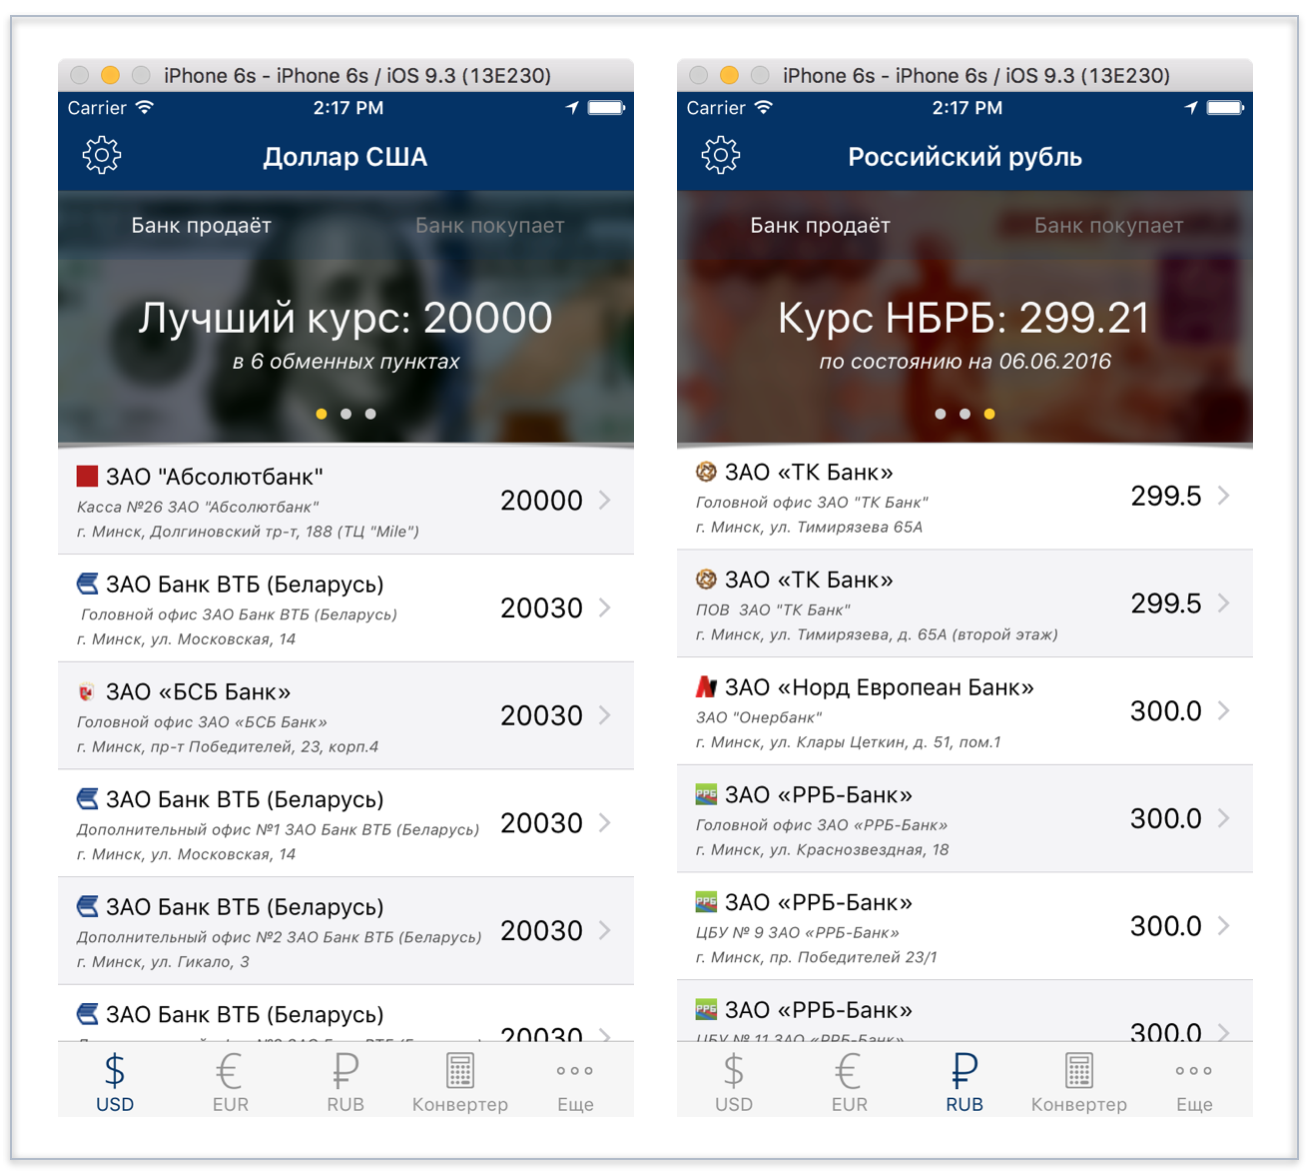
\includegraphics[width=120mm]{fig/main_screen_manual}
  \caption{Просмотр курсов валют на \\ главном экране приложения}
  \label{fig:main_screen_manual}
\end{figure}


% Просмотр детальной информации об отделении. Возможность открыть сайт, позвонить.

\paragraph{}

По нажатию на элемент списка открывается экран просмотра детальной информации
об отделении. На этом экране пользователь имеет возможность просмотреть название
банка, отделения, его контактную информацию. По нажатию на номер телефона
открывается стандартное для платформы iOS диалоговое окно,
предлагающее пользователю совершить вызов по выбранному номеру.
По нажатию на веб-сайт открывается браузер мобильного устройства.
Для возврата к списку отделений необходимо нажать на стрелку в левом верхнем
углу текущего экрана. Просмотр детальной информации о различных отделениях
коммерческих банков представлен на рисунке~\ref{fig:details_manual}.
\begin{figure}[h!]
  \centering
  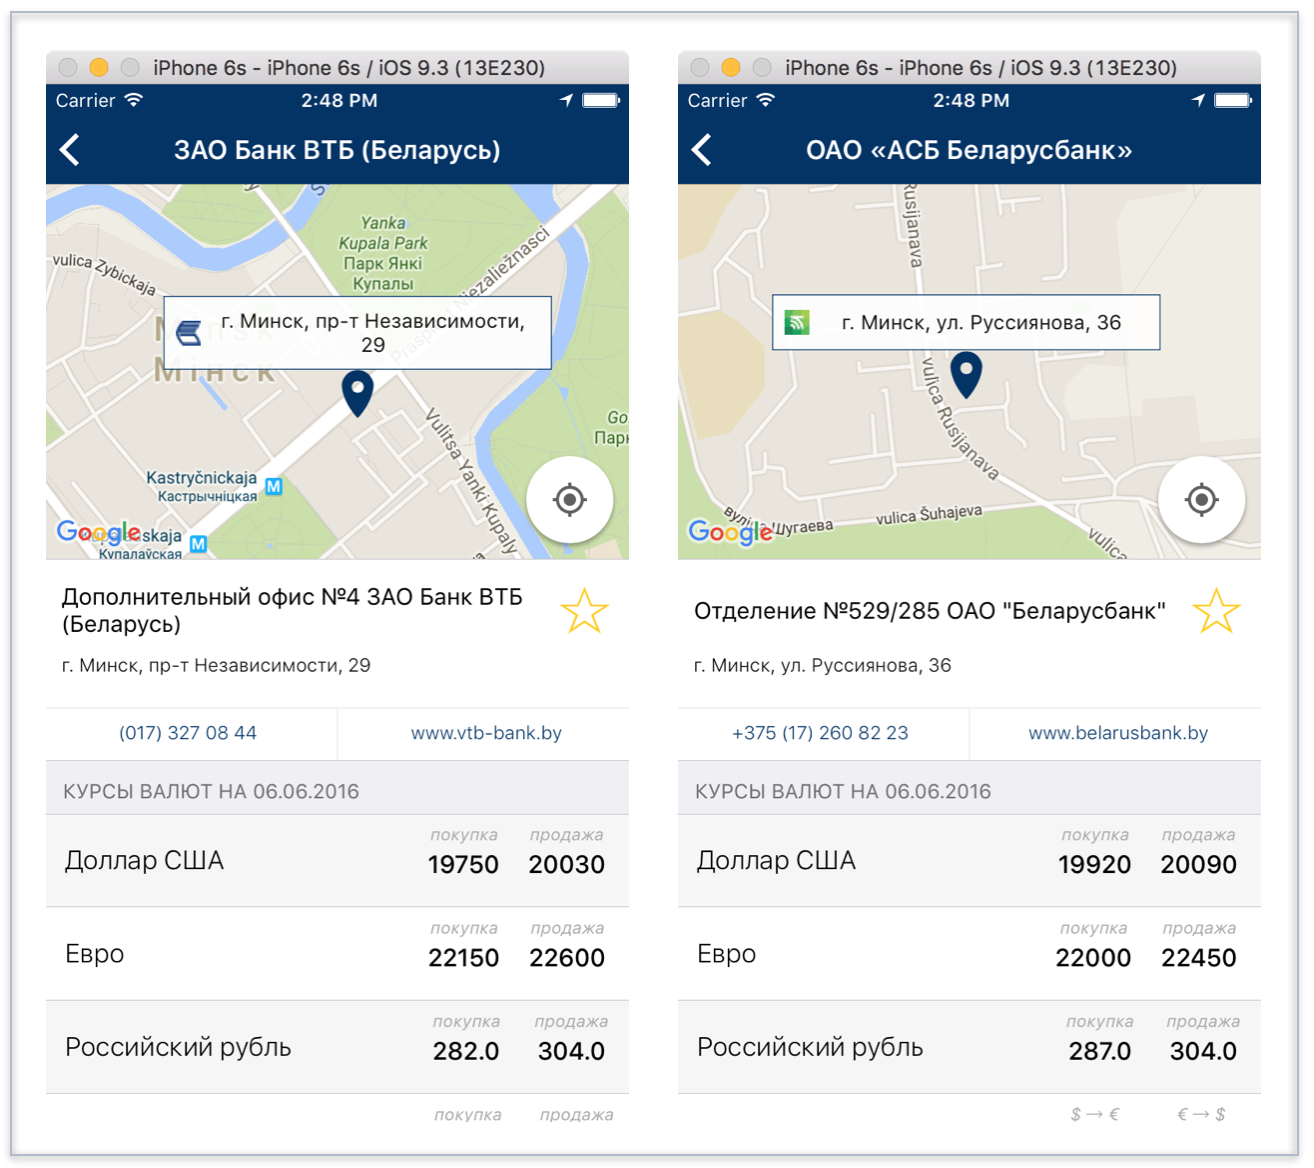
\includegraphics[width=140mm]{fig/details_manual}
  \caption{Просмотр детальной информации \\ о различных отделениях}
  \label{fig:details_manual}
\end{figure}


% Добавление отделения в избранное.

\paragraph{}

В приложении предусмотрена возможность добавления отделения в категорию <<Избранное>>.
Отделения, попадающие в эту категорию отображаются в верхней части списка
вне зависимости от выбранной пользователем валюты. Таким образом, пользователь
имеет возможность просмотреть контактную информацию, а также информацию о
курсах валют в конкретном отделении за кратчайшее время.

Для добавления отделения в избранное необходимо перейти на детальную информацию
об отделении, как это показано на рисунке~\ref{fig:details_manual}. По нажатию
на визуальный элемент <<Звезда>>, рассматриваемое отделение попадает
в категорию <<Избранное>>. Процес добавления отделение в избранное,
а также вариант просмотра отделений этой категории изображен
на рисунке~\ref{fig:favorite_manual}.
\begin{figure}[h!]
  \centering
  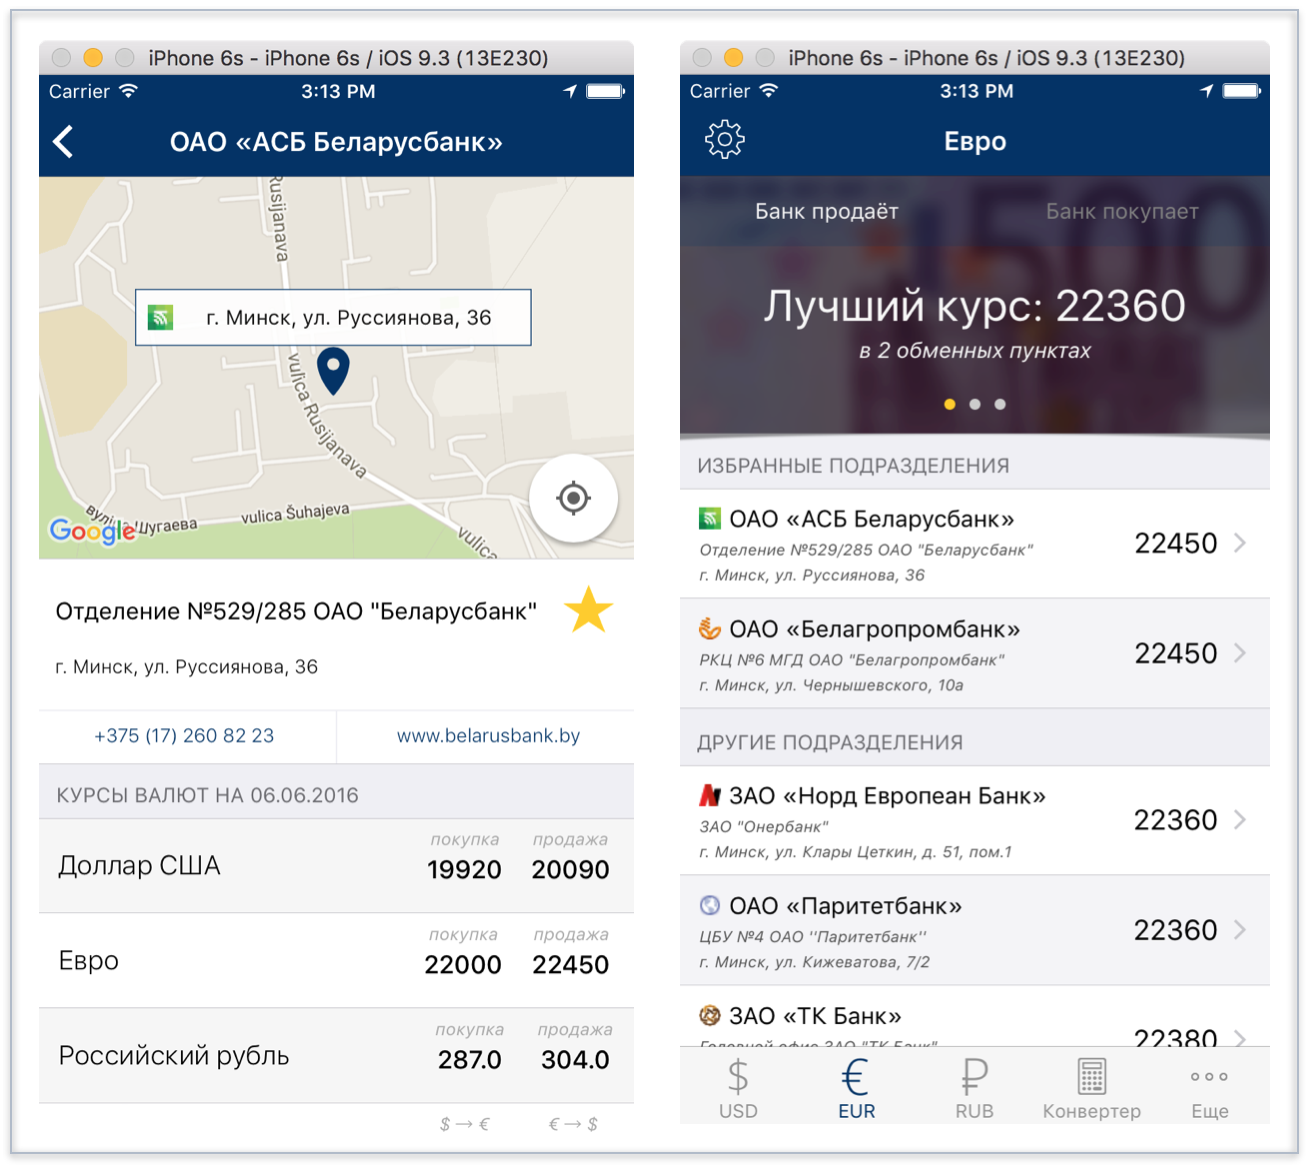
\includegraphics[width=140mm]{fig/favorite_manual}
  \caption{Избранные отделения коммерческих банков}
  \label{fig:favorite_manual}
\end{figure}


% Выполнение поиска.

\paragraph{}

В разрабатываемом приложении предусмотрена возможность использования поиска.
Поиск выполняется по нескольким параметрам: по названию отделения, банка,
а также по адресу. Например, пользователь имеет возможность найти отделения
коммерческих банков, находящиеся на определенной улице.

Для выполнения поиска необходимо открыть приложение. Находясь на главной странице,
выполнить сдвиг списка отделений жестом вниз. С использованием анимации движения
строка появится на экране устройства. По нажатию на строку поиска откроется
виртуальная клавиатура, которая позволит пользователю ввести необходимый запрос
для поиска отделения. После того, как пользователь ввёл в строке поиска
определенный запрос, следует перейти на экран поиска отделений. Для этого,
на виртуальной клавиатуре необходимо нажать кнопку <<Найти>>.
Пример поиска отделений, расположенных на улице Притыцкого города Минска
представлен на рисунке~\ref{fig:search_by_address_manual}.
\begin{figure}[h!]
  \centering
  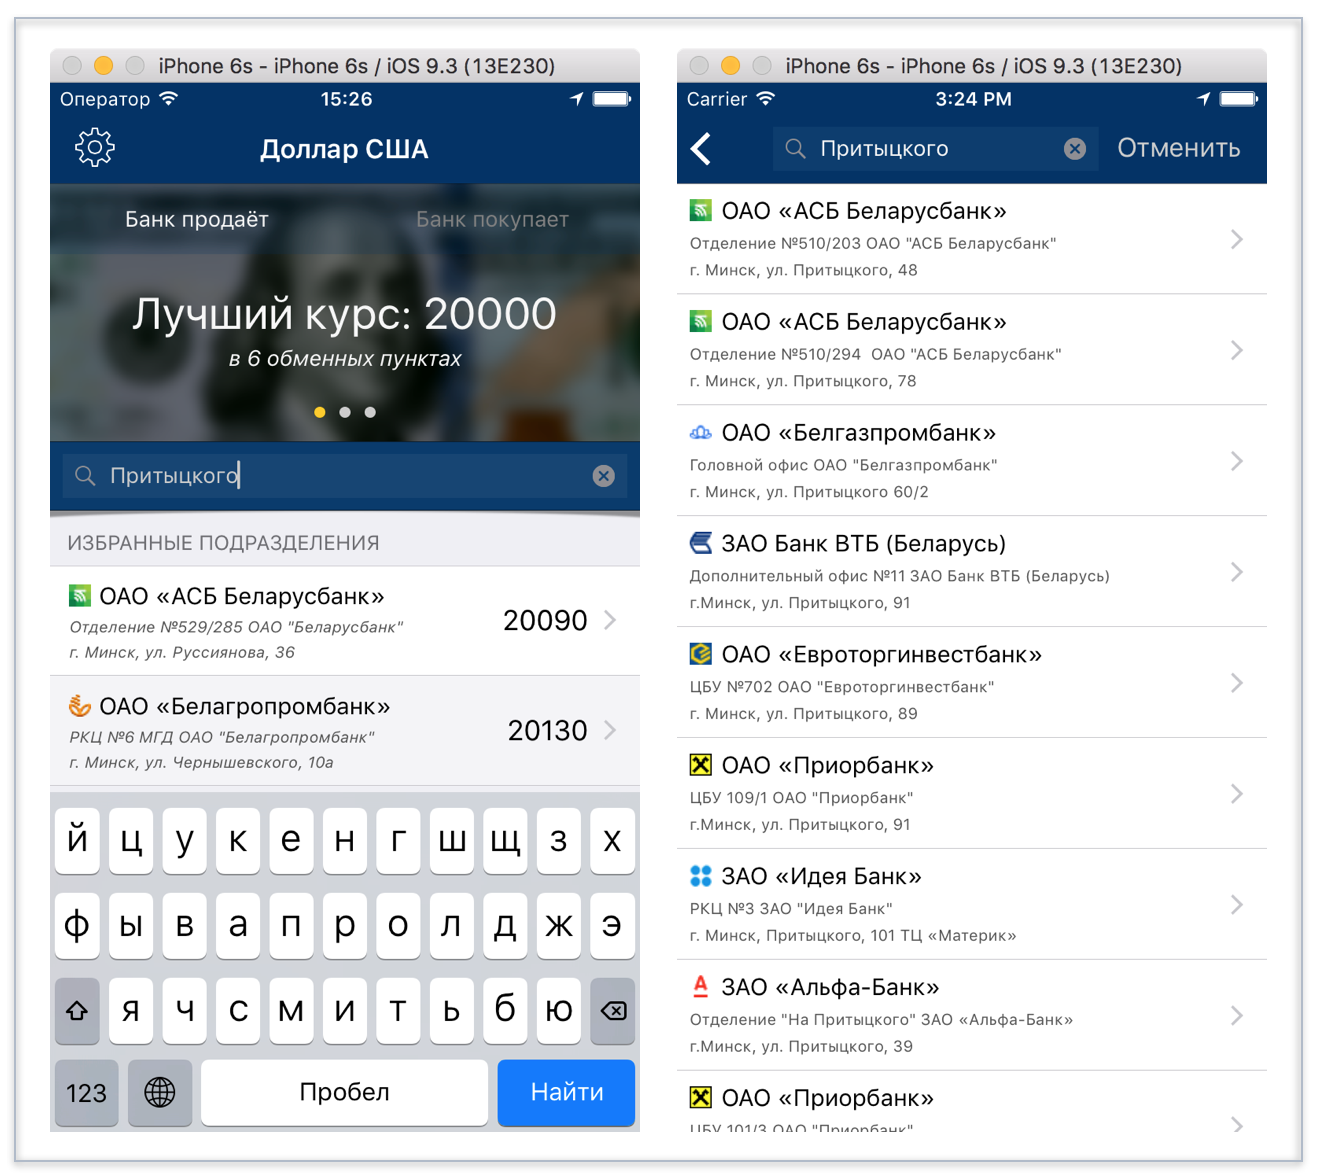
\includegraphics[width=140mm]{fig/search_by_address_manual}
  \caption{Пример поиска отделений \\ по запросу <<Притыцкого>>}
  \label{fig:search_by_address_manual}
\end{figure}


% Использование конвертера.

\paragraph{}

Пользователь имеет возможность использовать конвертер валют. Для этого,
находясь на главном экране приложения, необходимо нажать на кнопку <<Конвертер>>,
расположенную в нижней части экрана устройства. После этого будет открыт экран
конвертера валют. Пользователю доступно шесть полей для ввода, каждое из которых
соответствует определенной валюте и имеет подпись. При изменении значения в
любом из полей, значения во всех остальных полях будут автоматически пересчитаны.

Например, для конвертации 100 долларов США в другие валюты, в том числе
и в белорусские рубли, необходимо ввести значение <<100>> в поле с
надписью <<Доллар США>>. Для этого необходимо нажать на поле <<Доллар США>>.
После открытия виртуальной цифровой клавиатуры ввести значение <<100>>
и нажать кнопку <<Готово>>. При необходимости выполнения расчёта по курсу
Национального банка Республики Беларусь, требуется нажать на кнопку <<Курс НБРБ>>
в верхней правой части экрана. Пример использования конвертера валют приведен на
рисунке~\ref{fig:converter_manual}.
\begin{figure}[h!]
  \centering
  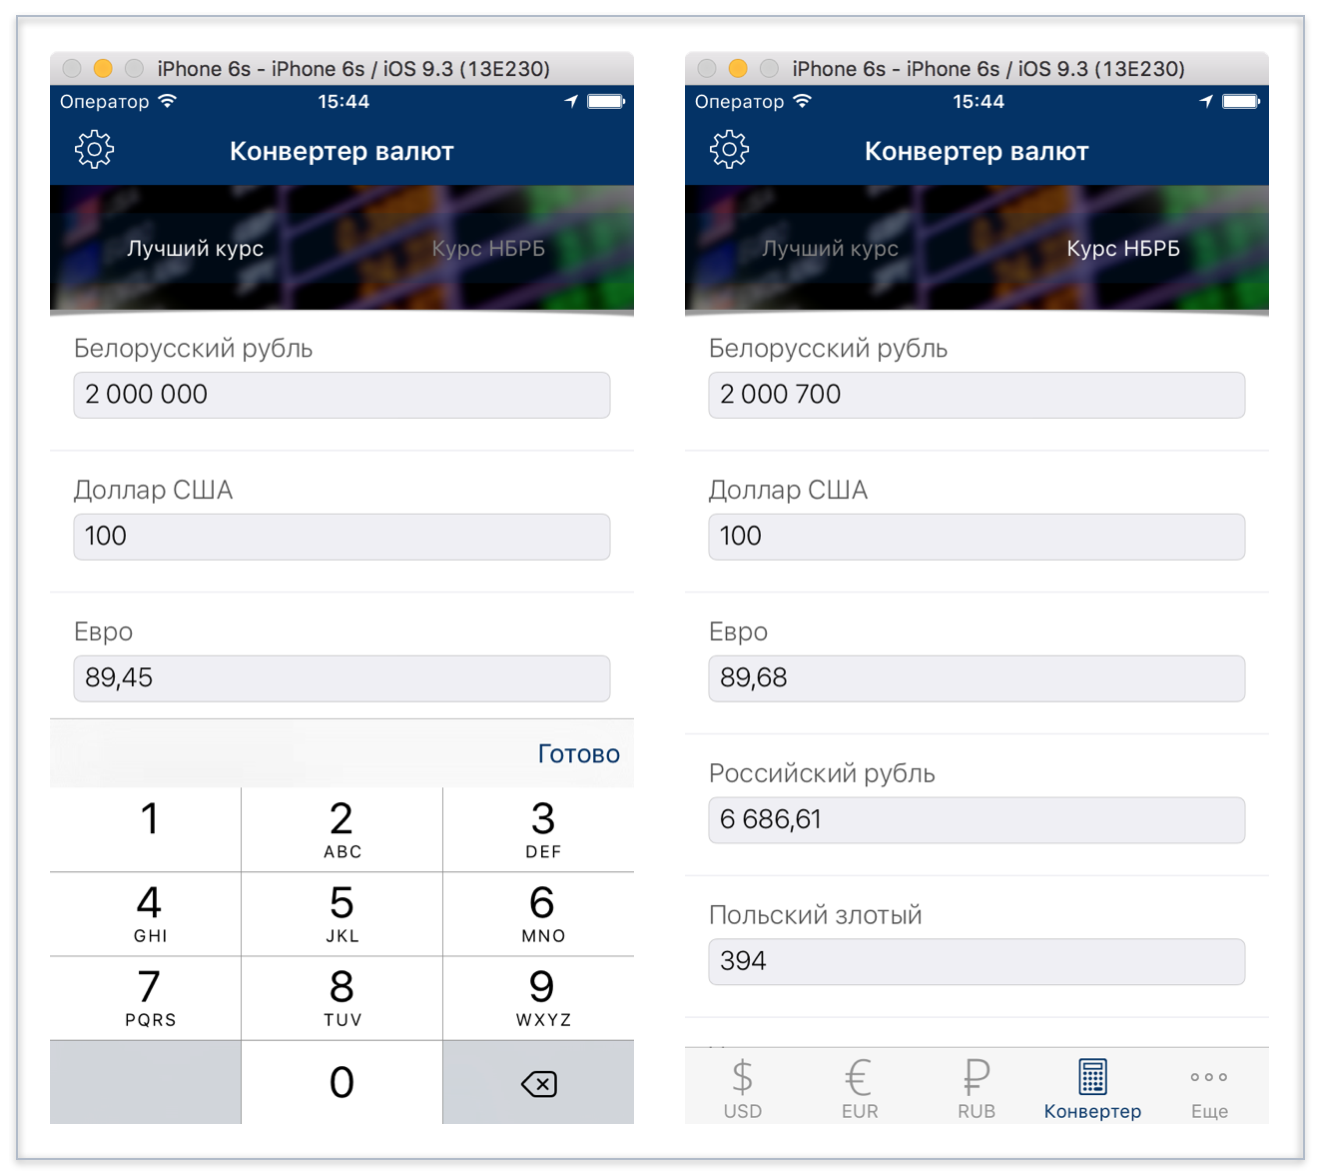
\includegraphics[width=150mm]{fig/converter_manual}
  \caption{Пример использования конвертера валют}
  \label{fig:converter_manual}
\end{figure}


% Изменение города в настройках приложения.

\paragraph{}

В разрабатываемом приложении предусмотрено получение финансовой информации в
зависимости от выбранного пользователем областного центра. Выбор города
выполняется пользователем в настройках приложения, значение по умолчанию ---
город Минск. Для того, чтобы просмотреть информацию о курсах валют в отличном
от выбранного областном центре, необходимо выполнить следующие действия:
\begin{enumerate}
  \item Находясь на главном экране приложения перейти в раздел настроек, нажав
    соответствующую кнопку в верхней левой части экрана мобильного устройства.
  \item Выбрать пункт меню <<Город>> с подписью <<Выберите город>>.
  \item В открывшемся списке нажатием выбрать необходимый областной центр.
  \item После сообщения об обновлении данных, нажать кнопку <<Готово>>
    в верхней левой части экрана.
\end{enumerate}

Пример изменения выбранного областного центра в настройках приложения приведен
на рисунке~\ref{fig:settings_manual}.
\begin{figure}[h!]
  \centering
  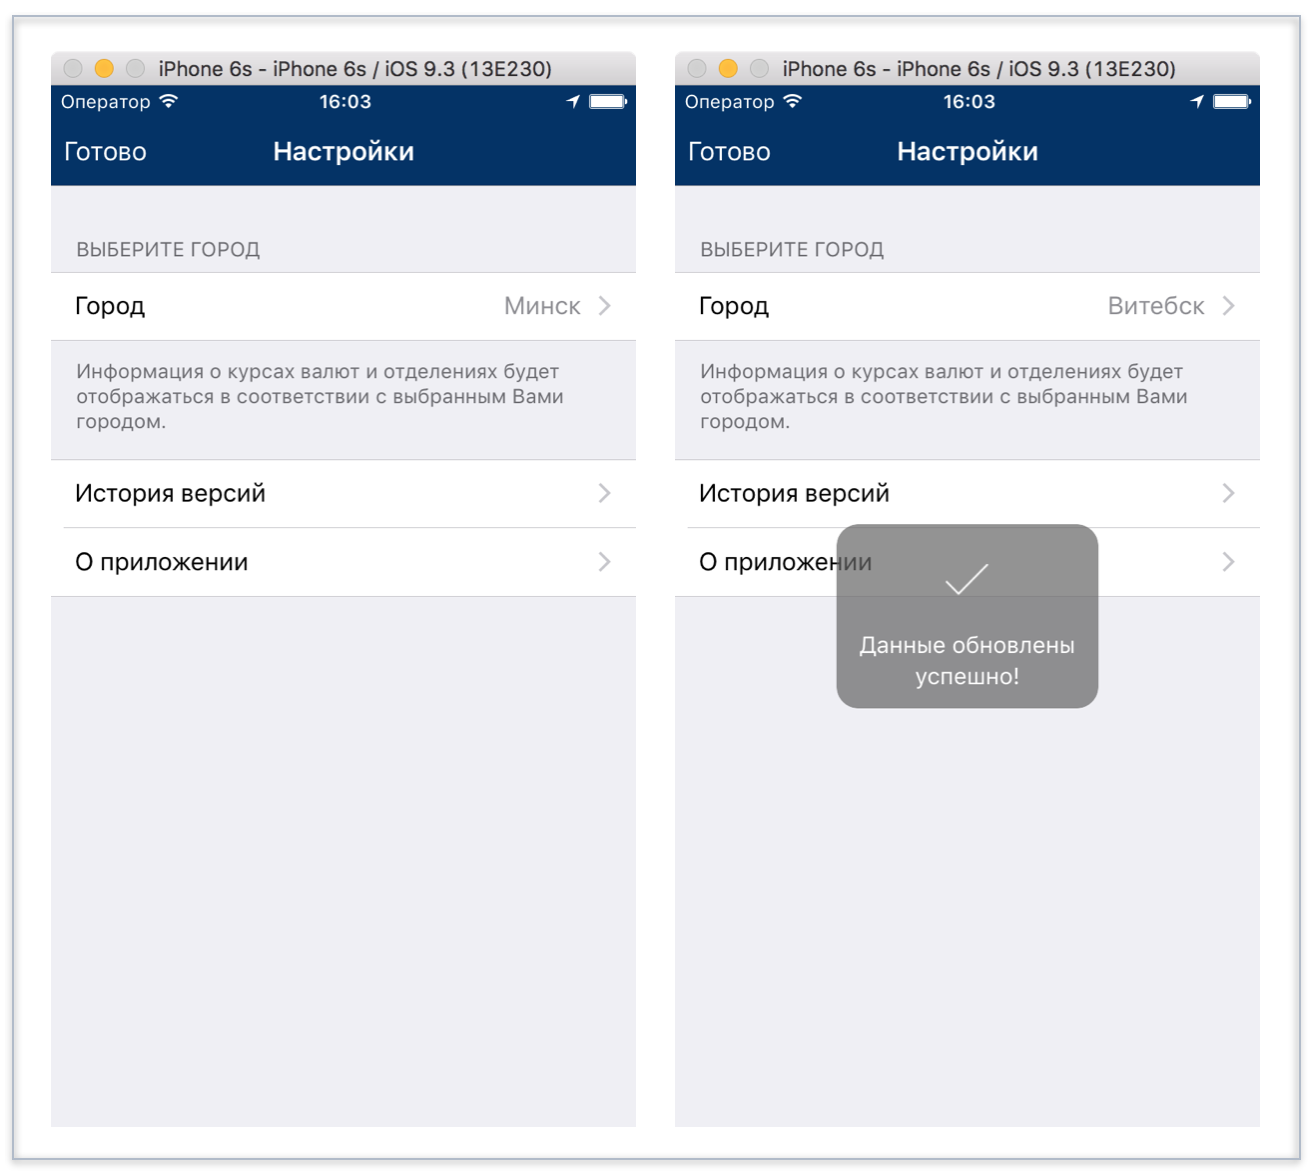
\includegraphics[width=130mm]{fig/settings_manual}
  \caption{Пример изменения областного центра \\ в настройках приложения}
  \label{fig:settings_manual}
\end{figure}

\pagebreak


% Перспективы развития

\subsection{Перспективы развития}

Для поддержания актуальности программного обеспечения, которое
создаётся для современных операционных систем, требуется выполнять его
регулярное обновление. Это связано с постоянным обновлением операционных систем,
изменением запросов пользователей, а также с желанием усовершенствовать
разработанное ПО.

Среднее время разработки мобильного приложения занимает 18
недель~\cite{time_to_develop_mobile_app}, что существенно влияет
на количество конкурентов в рамках предметной области разрабатываемого приложения.
Проанализировав возможности операционной системы iOS, а также функциональность,
предложенную приложениями-аналогами, можно выделить следующие направления развития
программного модуля:
\begin{enumerate}
  \item Использование карты для отображения множества отделений с использованием
    кластеризации.
  \item Интеграция локальных или \textit{Push}-уведомлений.
  \item Просмотр истории курсов валют, нанесение значений курсов валют на график.
\end{enumerate}

С 1 июля 2016 года в Республике Беларусь будет проведена деноминация официальной
денежной единицы --- белорусского рубля. Соответствующее решение принято Указом
Президента Республики Беларусь от 4 ноября 2015 года № 450.
Деноминация будет проведена путем замены находящихся в обращении банкнот
образца 2000 года на банкноты и монеты образца 2009 года в соотношении 10 000 белорусских
рублей в денежных знаках образца 2000 года к одному белорусскому рублю в денежных
знаках образца 2009 года~\cite{denomination_decree, denomination_news}.

Проведение деноминации повлечет за собой большой объём работы в области
тестирования разработанного программного модуля и отладки в соответствие с
обновленным форматом входных данных.
